\begin{figure*}[ht]
\centering
    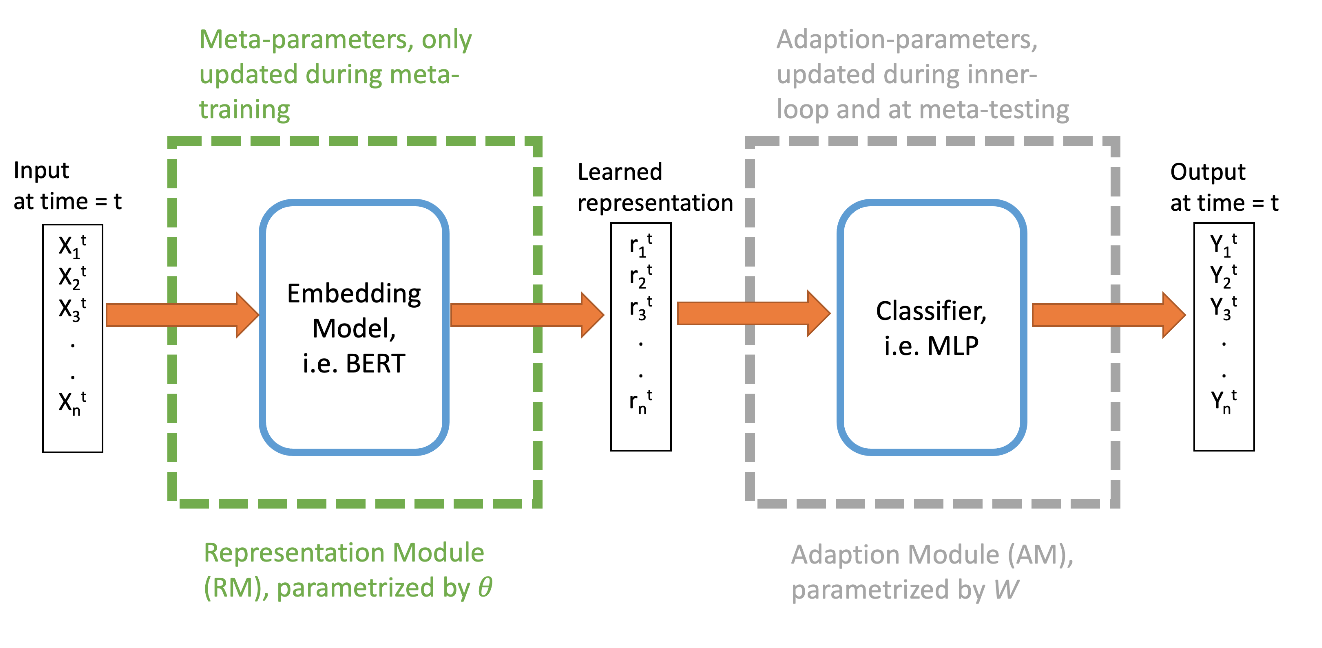
\includegraphics[scale=0.6]{imgs/framework.jpg}
    \caption{Our proposed framework composed of two modules: Representation Module and Adaption Module}
    \label{img:1}
\end{figure*}


At first, introduce some Automatic Content Extraction (ACE) terminologies to help understand the Event Detection tasks \citep{cao2020incremental}: "\textbf{Event trigger} refers to a word that most clearly expresses the occurrence of an event. \textbf{Event arguments} are participants of the event. \textbf{Event mention} refers to a phrase or sentence within which an event is described."

Because Continual Event Detection (CED) in Natural Language problem can be viewed as a kind of Continual Learning Prediction (CLP), this paper, which majorly exploits meta-learning based methods, formulate the CED problem based on the CLP problem formulation from \citet{javed2019meta}.
A Continual Event Detection (CED) in Natural Language problem consists of an endless data stream:
\[\mathcal{T} = (X_1, Y_1), (X_2, Y_2), \dots, (X_t, Y_t), \dots\]
for inputs $X_t$ (event mentions) and targets $Y_t$ (event types), from sets $\mathcal{X}$ and $\mathcal{Y}$. The random vector $Y_t$ is sampled
according to an unknown distribution $p(Y|X_t)$. We define $S_k = (X_j+1, Y_j+1), (X_j+2, Y_j+2), \dots, (X_j+k, Y_j+k)$ as a trajectory of length k which is smapled randomly from the CET problem $\mathcal{T}$, and $p(S_k|\mathcal{T})$ represents a distribution over all the trajectories $S_k$.

Our goal is to learn a function $f_W,\theta$ which predict $Y_t$ for $X_t$, and minimize the loss function below for a CED problem:
\begin{equation}
    \begin{split}
    &\mathcal{L}_{C E D}(W, \theta)  \\
    &\stackrel{\text { def }}{=}  \mathbb{E}\left[\ell\left(f_{W, \theta}(X), Y\right)\right] \\ 
    & =\int\left[\int \ell\left(f_{W, \theta}(x), y\right) p(y \mid x) d y\right] \mu(x) d x
    \end{split}
\end{equation}
where $W$ and $\theta$ are the parameters to be updated to minimize the objective $\mathcal{L}_{C E D}$.
